\documentclass[12pt,a4paper]{article}
\usepackage[top=1 in,  bottom=1 in, left=1 in, right=1 in]{geometry}
\usepackage{amsfonts,amssymb,amsmath}
\usepackage{graphicx}
\usepackage{hyperref}
\usepackage{color}
%\usepackage{tikz}
%\usepackage[siunitx]{circuitikz}
%\usepackage{cite}
\usepackage{caption}
\usepackage{subcaption}
\usepackage{rotating}
\usepackage{paralist}
\usepackage{cprotect}

\definecolor{red}{rgb}{1, 0, 0}   %used for making comments in red color text
\definecolor{green}{rgb}{0, 0.7, 0}
\definecolor{blue}{rgb}{0, 0, 1}
\newcommand{\mc}{\textcolor{red}}  %used for making comments in red color text remove before submit
\newcommand{\mg}{\textcolor{green}}  %used for making comments in red color text remove before submit
\newcommand{\mb}{\textcolor{blue}}  %used for making comments in red color text remove before submit
\newcommand{\comment}[1]{}  %used for commenting out blocks of text remove before submit
\newcommand{\pyb}[1]{} % do nothing command for marking for python extraction
\newcommand{\pye}{} % do nothing command for python extraction end


\begin{document}
\author{Thomas Aref}
%\inst{3} {Department of Microtechnology and Nanoscience (MC2), Chalmers University of Technology, SE-412 96 G\"oteborg, Sweden}
\title{Sample TA210715A46 in Speedy 3-10-15 cooldown}
\maketitle
\noindent
\pyb {summary}
    \section{SASDy}
    This is an attempt at reducing the coupling by changing the spacing of the fingers pairs on the qubit IDT, pus

\pye

\pyb {second entry}
this is the second entry
\pye

\subsection{Qubit values}
\begin{tabular}{|p{5 cm}|p{3 cm}|}
\hline
 Qubit & {} \\
\hline
 Finger type & double finger \\
\hline
 Number of finger pairs, $N_{pq}$ & 9 \\
\hline
 Overlap length, $W$ & 25 $\mu$m \\
\hline
 finger width, $a_q$ & 80 nm \\
\hline
 DC Junction Resistances & 8.93 k$\Omega$, 9.35k$\Omega$ \\
\hline
 Metallization ratio & 50\% \\
\hline
\end{tabular}

\setcounter{subfigure}{0} % reset figure counter to 0.
\begin{figure}[ht!]
\centering
\begin{subfigure}[b]{0.49\textwidth}
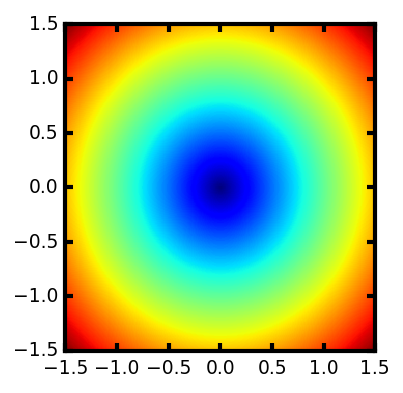
\includegraphics[width=\textwidth]{test_colormap_plot.png}
\end{subfigure}
\label{fig:setup}
\cprotect\caption{Analysis: \verb;/TA_software/taref/tex/tex.py;}
\end{figure}
\end{document}